\section{Coeficientes CAPECO}

\subsection{Coeficientes CAPECO originales - 2001}

\begin{table}[h!]
	\small
	\centering
	\caption{Tabla de coeficientes de Condición de Percepción según edad región y sexo utilizados para la construcción de CAPECO 2001}
	\label{tab:tableCP2001}
	\begin{tabular}{|c|c|c|c|c|}
		\hline
		\multicolumn{2}{|c|}{} & \multicolumn{3}{|c|}{Edad} \\
		\hline
		\multicolumn{2}{|c|}{Ocupados} & 14-24 años & 25-34 años & 35 años y más \\
		\hline
		Varones & GBA & 0.46 & 0.83 & 1.00	\\
		        & NOA & 0.32 & 0.49 & 0.67	\\	
		        & NEA & 0.26 & 0.46 & 0.65	\\	
		        & Cuyo & 0.32 & 0.52 & 0.68	\\
		        & Pampeana & 0.39 & 0.62 & 0.81	\\
		        & Patagonia & 0.60 & 1.00 & 1.27	\\
		\hline
		Mujeres & GBA & 0.33 & 0.54 & 0.60	\\
				& NOA & 0.22 & 0.31 & 0.43	\\	
				& NEA & 0.20 & 0.30 & 0.44	\\	
				& Cuyo & 0.25 & 0.32 & 0.41	\\
				& Pampeana & 0.25 & 0.40 & 0.50	\\
				& Patagonia & 0.44 & 0.58 & 0.71	\\
		\hline
		\multicolumn{5}{|l|}{Jubilados}\\
		\hline
		\multicolumn{2}{|l|}{Varones} & \multicolumn{3}{|c|}{0.50}\\
		\multicolumn{2}{|l|}{Mujeres} & \multicolumn{3}{|c|}{0.35}\\
		\hline   
		\multicolumn{5}{|l|}{Desocupados, estudiantes, otra ocupación}\\
		\hline
		\multicolumn{5}{|c|}{0.00}\\
		
	\end{tabular}
\end{table}

\begin{table}[h!]
	\small
	\centering
	\caption{Tabla de transformación de los años de escolaridad aprobados respecto del valor en el mercado laboral del séptimo año de educación de un varón de 35 años y más de GBA. CAPECO 2001}
	\label{tab:tableVAE2001}
	\begin{tabular}{p{1cm}|p{3cm}}
		Años aprobados & Valor de los años de escolaridad aprobados
		reescalados al individuo testigo \\
		\hline
		0 & 4,0\\
		\hline
		1 & 4,4\\
		\hline
		2 & 4,7\\
		\hline
		3 & 5,1\\
		\hline
		4 & 5,5\\
		\hline
		5 & 6,0\\
		\hline
		6 & 6,5\\
		\hline
		7 & 7,0\\
		\hline
		8 & 7,7\\
		\hline
		9 & 8,4\\
		\hline
		10 & 9,2\\
		\hline
		11 & 10,1\\
		\hline
		12 & 11,1\\
		\hline
		13 & 12,6\\
		\hline
		14 & 14,4\\
		\hline
		15 & 16,4\\
		\hline
		16 & 18,6\\
		\hline
		17 & 21,2\\
		
	\end{tabular}
\end{table}

\begin{table}[h!]
	\small
	\centering
	\label{tab:tableAE2001}
	\caption{Tabla de escala de adulto equivalente utilizados para la construcción de CAPECO 2001}
	\begin{tabular}{p{2cm}|p{6cm}}
		Valor en unidades de adulto equivalente & Características de sexo y edad \\
		\hline
		0.33&Niños de ambos sexos menores de un año de edad\\
		\hline		
		0.43&Niños de ambos sexos de 1 año de edad\\
		\hline		
		0.5&Niños de ambos sexos de 2 años de edad\\
		\hline		
		0.56&Niños de ambos sexos de 3 años de edad\\
		\hline		
		0.63&Niños de ambos sexo entre 4 y 6 años de edad\\
		\hline		
		0.72&Niños de ambos sexos entre 7 y 9 años de edad\\
		\hline		
		0.83&Varones entre 10 y 12 años de edad\\
		\hline		
		0.96&Varones entre 13 y 15 años de edad\\
		\hline		
		1.05&Varones entre 16 y 17 años de edad\\
		\hline		
		0.73&Mujeres entre 10 y 12 años de edad\\
		\hline		
		0.79&Mujeres entre 13 y 15 años de edad\\
		\hline		
		0.79&Mujeres entre 16 y 17 años de edad\\
		\hline		
		1.06&Varones entre 18 y 29 años de edad\\
		\hline		
		1.00&Varones entre 30 y 59 años de edad\\
		\hline		
		0.82&Varones de 60 y más años de edad\\
		\hline		
		0.74&Mujeres entre 18 y 29 años de edad\\
		\hline		
		0.74&Mujeres entre 30 y 59 años de edad\\
		\hline		
		0.64&Mujeres de 60 y más años de edad\\
	\end{tabular}
\end{table}


\subsection{Coeficientes CAPECO actualizado - 2010}

\subsection{Adulto equivalente CAPECO original - 2001}\label{anexo}

\section{Cuadros y gráficos adicionales}

 \begin{figure}[!htb]
 	\textbf{Ingreso (ln) según género y escolaridad - Mujeres}\par\medskip
 	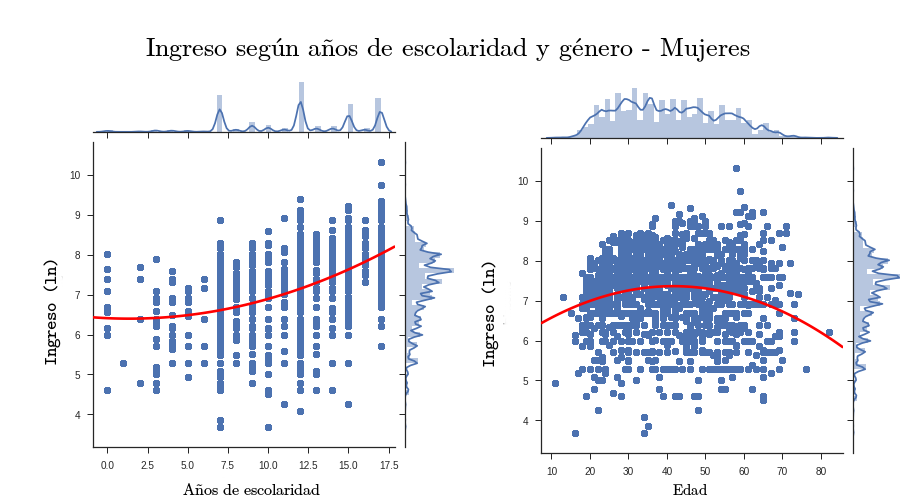
\includegraphics[scale = 0.4]{../img/capitulo3/ingresoVedadVescolaridadMujeres.png}
 	\caption{.}
 	\label{fig:ingresoVedadVescolaridadMujeres}
 \end{figure}
 
 \begin{figure}[!htb]
 	\textbf{Ingreso (ln) según género y escolaridad - Varones}\par\medskip
 	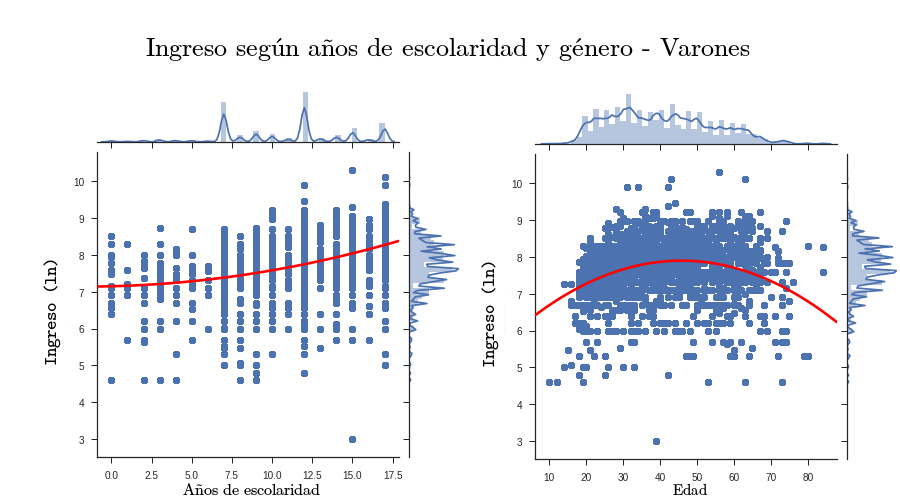
\includegraphics[scale = 0.4]{../img/capitulo3/ingresoVedadVescolaridadVarones.png}
 	\caption{.}
 	 \label{fig:ingresoVedadVescolaridadVarones}
 \end{figure}
